\chapter{(Continuous) Uniform Distribution ($X \sim \mathcal{U}(\theta_0,\theta_1)$) \cite{ism-1,wiki/Continuous_uniform_distribution}} \label{Uniform Distribution}

\begin{table}[H]
    \begin{minipage}{0.49\linewidth}
        \begin{figure}[H]
            \centering
            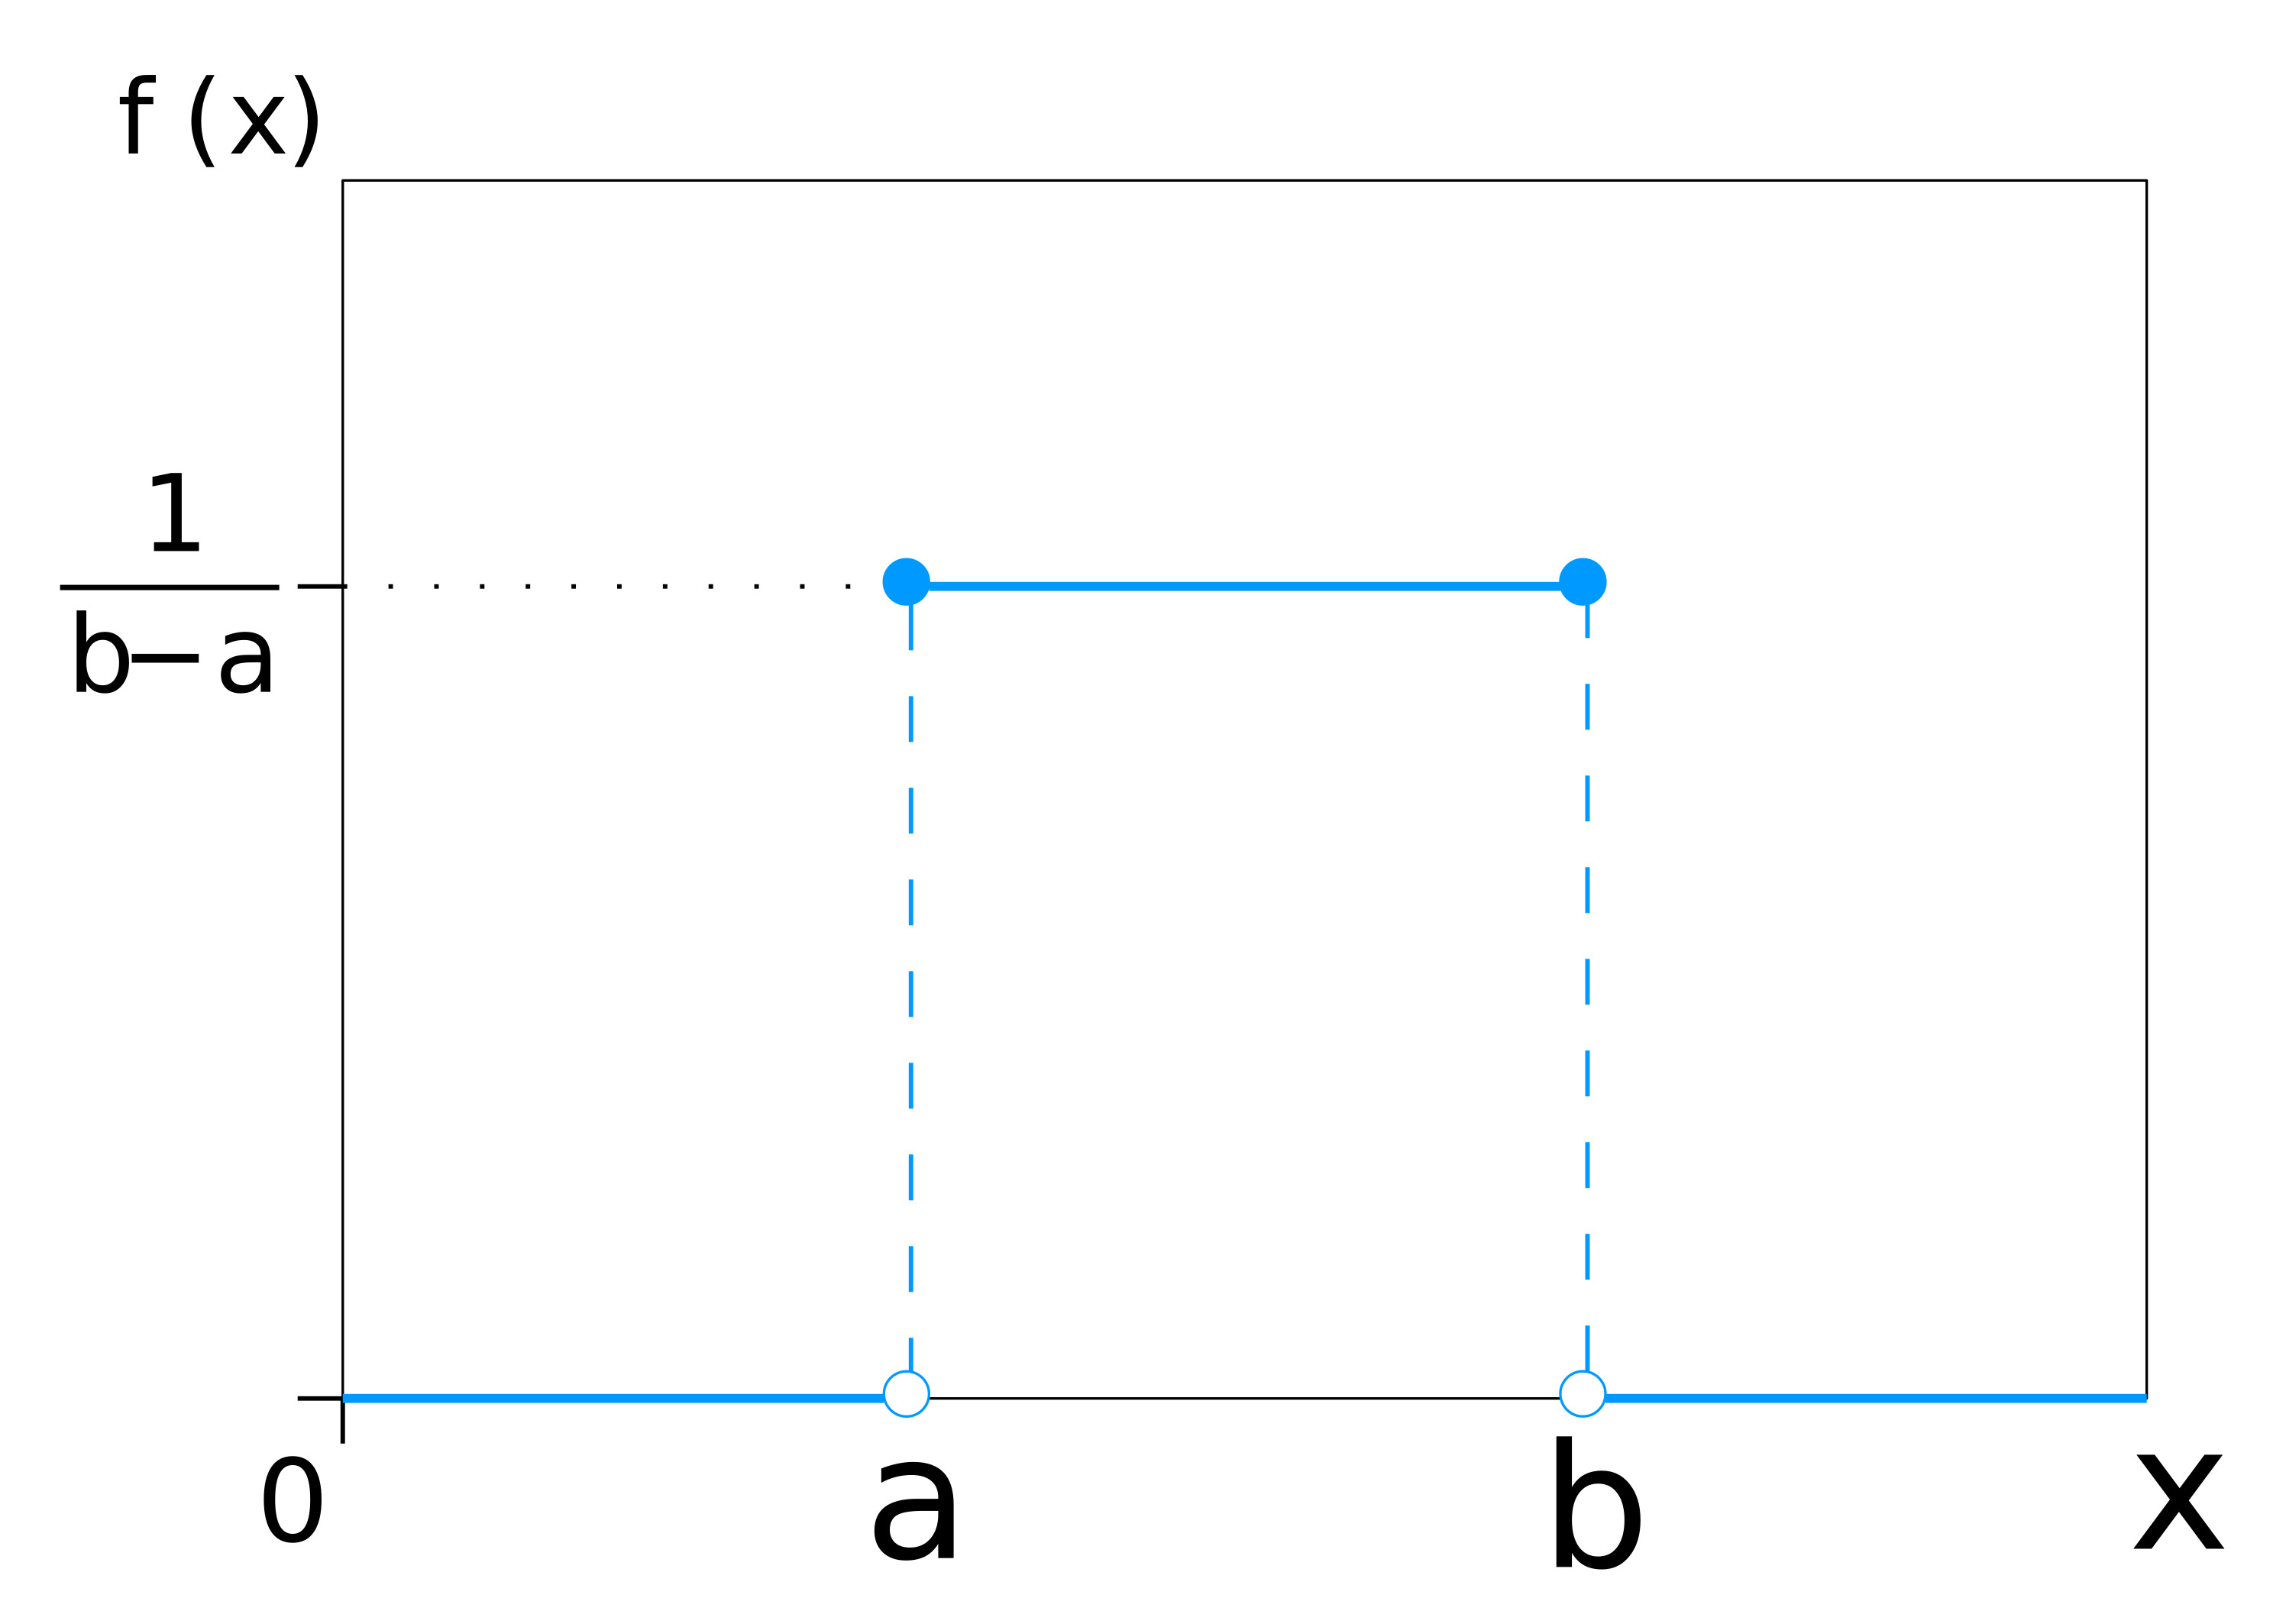
\includegraphics[width=\linewidth, height=4cm, keepaspectratio]{Pictures/distributions/Uniform_Distribution_PDF.jpg}
            \caption{(Continuous) Uniform Distribution: PDF}
        \end{figure}
    \end{minipage}
    \hfill
    \begin{minipage}{0.49\linewidth}
        \begin{figure}[H]
            \centering
            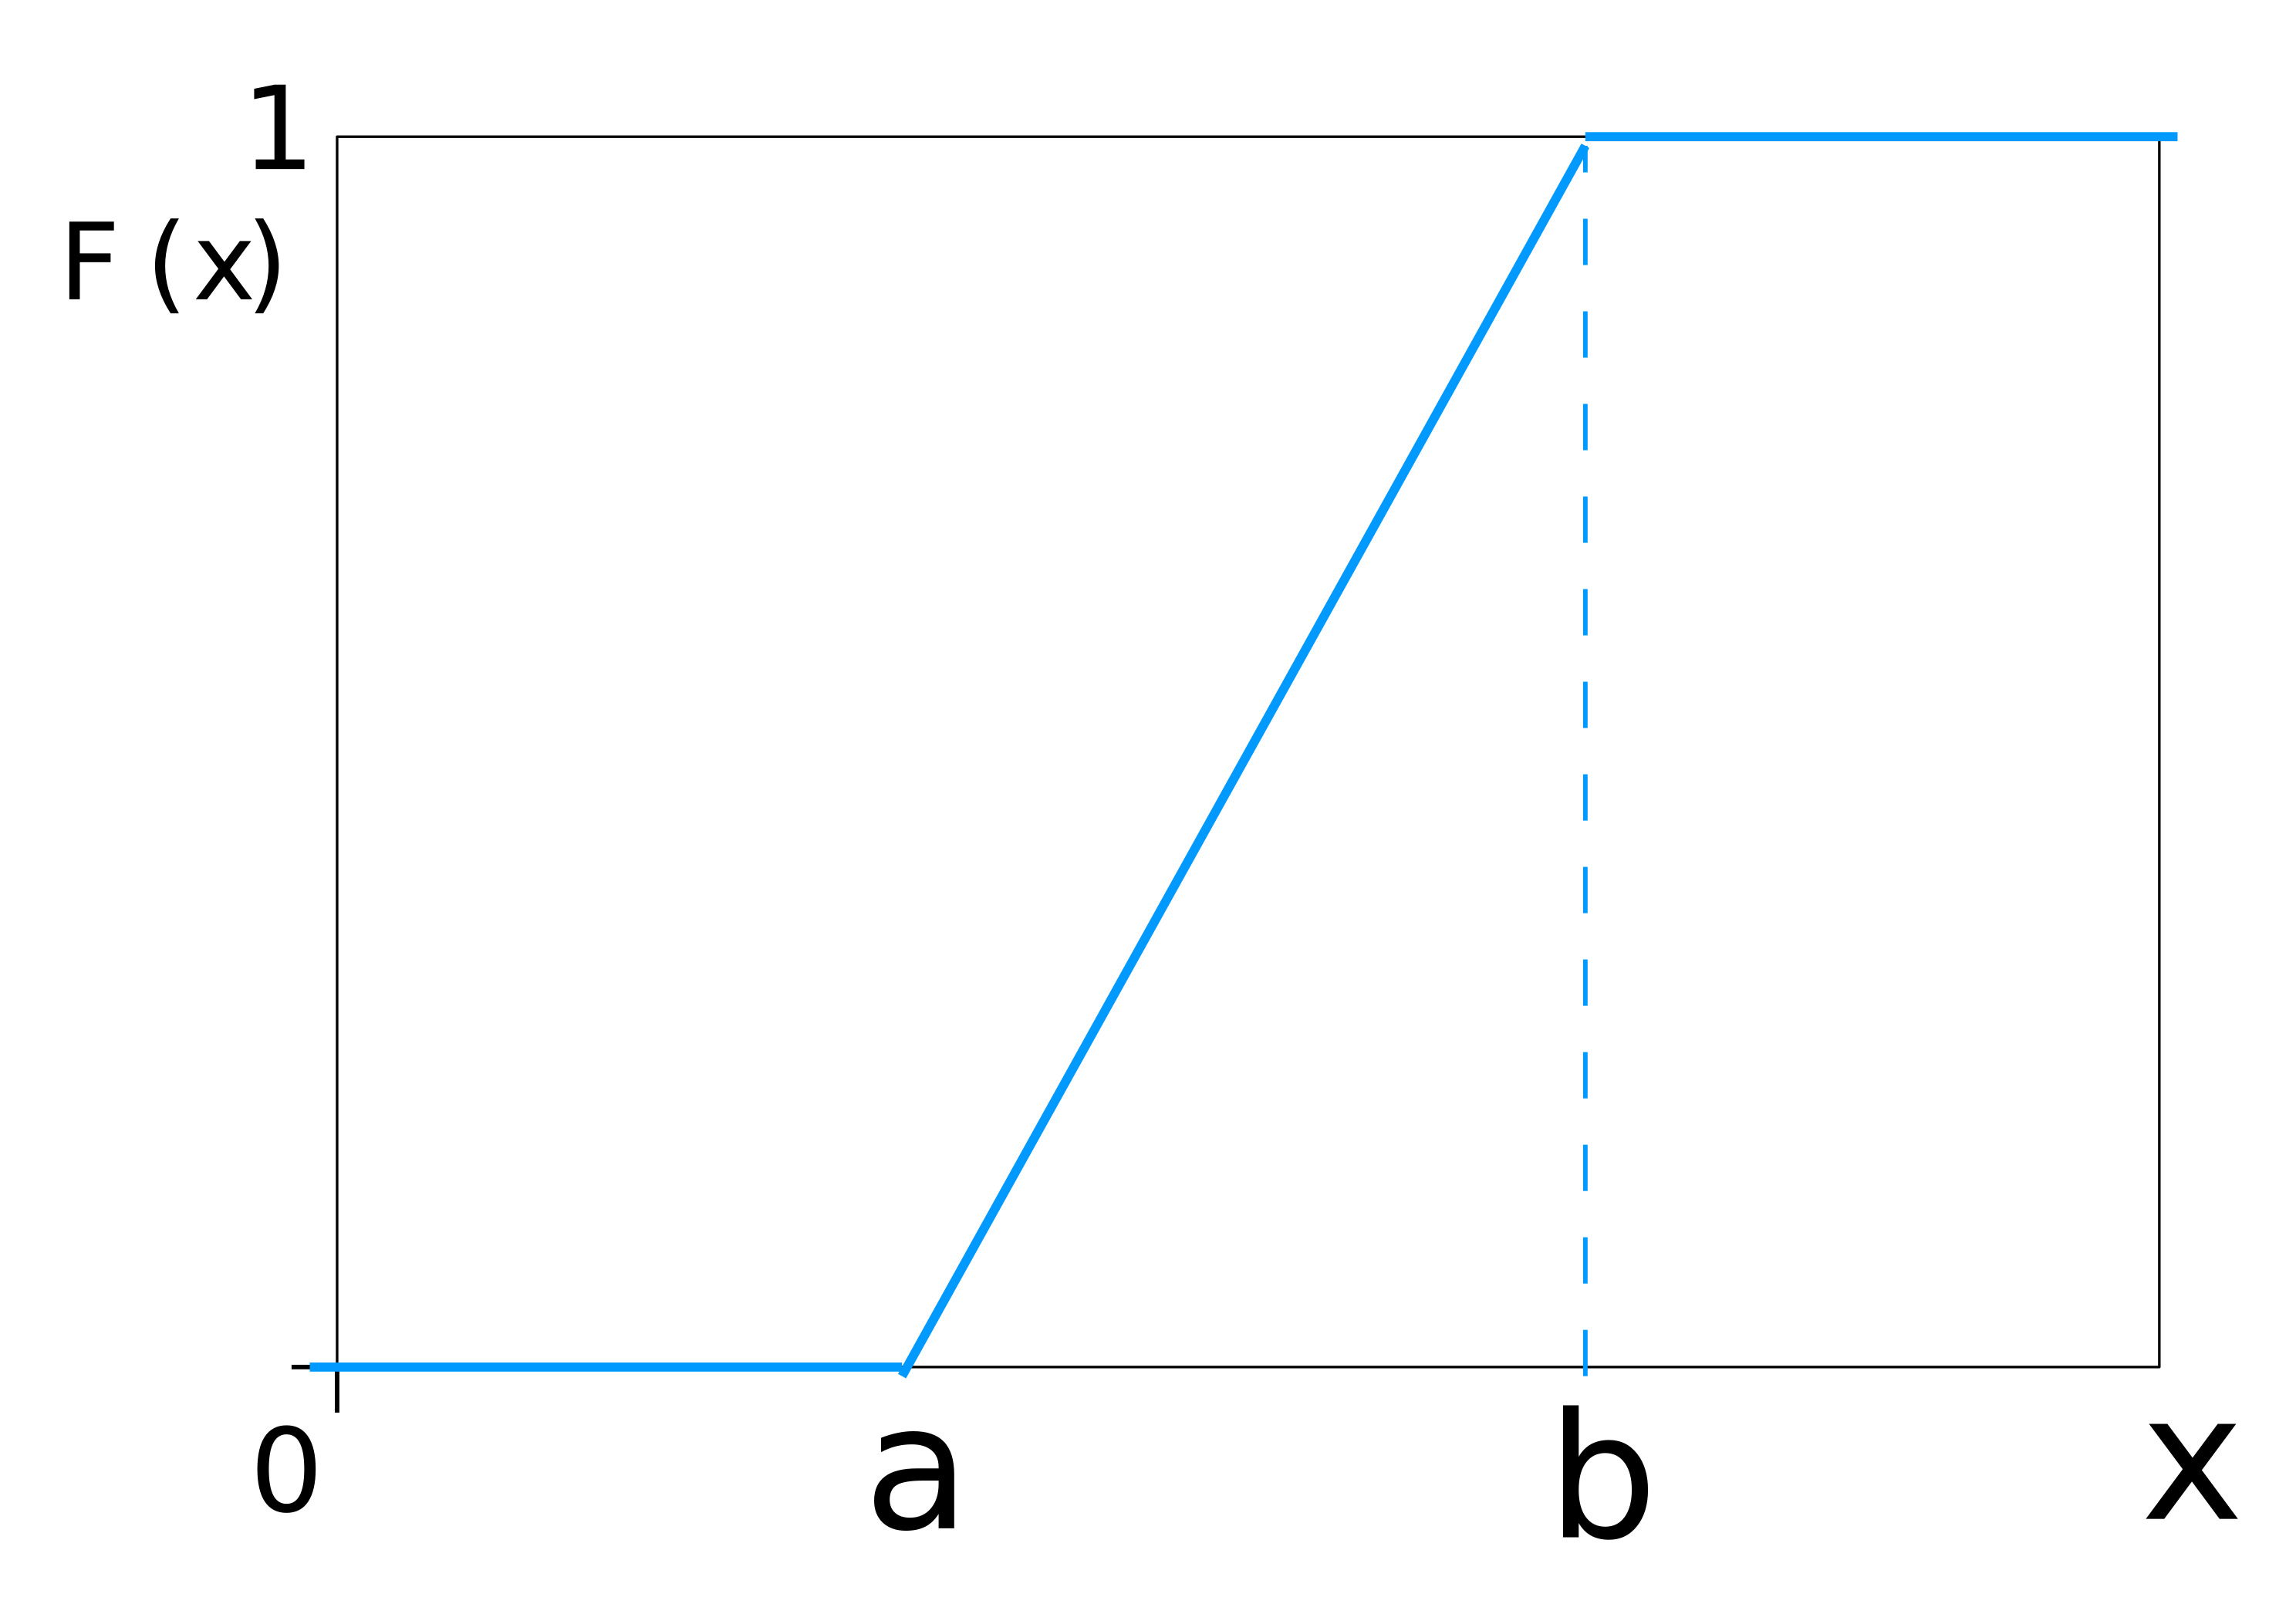
\includegraphics[width=\linewidth, height=4cm, keepaspectratio]{Pictures/distributions/Uniform_Distribution_CDF.jpg}
            \caption{(Continuous) Uniform Distribution: CDF}
        \end{figure}
    \end{minipage}
\end{table}

$\hfill a = \theta_0$ \hfill \& \hfill $b = \theta_1 \hfill$

\begin{customTableWrapper}{2}
\begin{longtable}{|m{6cm}|p{9cm}|}
    \hline
    \customTableHeaderColor
    \multicolumn{2}{|c|}{\textbf{(Continuous) Uniform Distribution - Info} \cite{wiki/Continuous_uniform_distribution}} \\
    \hline\endfirsthead

    \hline
    \customTableHeaderColor
    \multicolumn{2}{|c|}{\textbf{(Continuous) Uniform Distribution - Info - contd.} \cite{wiki/Continuous_uniform_distribution}} \\
    \hline\endhead
    
    \hline\endfoot
    \hline\endlastfoot

    \hline
    \textbf{Notation} & 
    ${\displaystyle {\mathcal {U}}_{[\theta_0,\theta_1]}}$
    \\ \hline

    \textbf{Statistical parameters} & 
    ${\displaystyle -\infty <\theta_0<\theta_1<\infty }$
    \\ \hline
    
    \textbf{Support} & 
    ${\displaystyle [\theta_0,\theta_1]}$
    \\ \hline

    \textbf{Probability Density Function (PDF)} & 
    ${\displaystyle {\begin{dcases}{\dfrac {1}{\theta_1-\theta_0}}&{\text{for }}x\in [\theta_0,\theta_1]\\0&{\text{otherwise}}\end{dcases}}}$
    \\[2ex] \hline
    
    \textbf{Cumulative distribution function (CDF)} & 
    ${\displaystyle {\begin{dcases}0&{\text{for }}x<\theta_0\\{\dfrac {x-\theta_0}{\theta_1-\theta_0}}&{\text{for }}x\in [\theta_0,\theta_1]\\1&{\text{for }}x>\theta_1\end{dcases}}}$
    \\ \hline

    \textbf{Mean} & 
    ${\displaystyle {\dfrac {1}{2}}(\theta_0+\theta_1)}$
    \\[1ex] \hline

    \textbf{Median} & 
    ${\displaystyle {\dfrac {1}{2}}(\theta_0+\theta_1)}$
    \\[1ex] \hline

    \textbf{Mode} & 
    ${\displaystyle {\text{any value in }}(\theta_0,\theta_1)}$
    \\ \hline

    \textbf{Variance} &
    ${\displaystyle {\dfrac {1}{12}}(\theta_1-\theta_0)^{2}}$
    \\[1ex] \hline

    \textbf{Mean absolute deviation (MAD)} &
    ${\displaystyle {\dfrac {1}{4}}(\theta_1-\theta_0)}$
    \\[1ex] \hline

    \textbf{Skewness} &
    $0$
    \\ \hline

    \textbf{Excess kurtosis} &
    ${\displaystyle -{\dfrac {6}{5}}}$
    \\[1ex] \hline

    \textbf{Entropy} &
    ${\displaystyle \log(\theta_1-\theta_0)}$
    \\[1ex] \hline

    \textbf{Moment-generating function (MGF)} &
    ${\displaystyle {\begin{dcases}{\dfrac {\mathrm {e} ^{t\theta_1}-\mathrm {e} ^{t\theta_0}}{t(\theta_1-\theta_0)}}&{\text{for }}t\neq 0\\1&{\text{for }}t=0\end{dcases}}}$
    \\[1ex] \hline

    \textbf{Characteristic function (CF)} &
    ${\displaystyle {\begin{dcases}{\dfrac {\mathrm {e} ^{\mathrm {i} t\theta_1}-\mathrm {e} ^{\mathrm {i} t\theta_0}}{\mathrm {i} t(\theta_1-\theta_0)}}&{\text{for }}t\neq 0\\1&{\text{for }}t=0\end{dcases}}}$
    \\[1ex] \hline

\end{longtable}
\end{customTableWrapper}


Parameters:
\begin{enumerate}
    \item $\theta_0$ : minimum value of population, $\theta_1$ : maximum value of population

    \item 
        \hfill
        $\theta_0 < \theta_1$
        \hfill
        $\theta_0 \leq x \leq \theta_1$
        \hfill

\end{enumerate}



\section{(Continuous) Standard Uniform Distribution ($X \sim \mathcal{U}(0,1)$) \cite{ism-1}} \label{Standard Uniform Distribution}

\begin{enumerate}
    \item $\theta_0 = 0$ and $\theta_1 = 1$

\end{enumerate}

























